
\documentclass[nototal]{beamer}
\mode<presentation>
{
  \usetheme{Madrid}
  \setbeamercovered{transparent}
}

\usepackage{verbatim}
\usepackage{fancyvrb}
\usepackage[english]{babel}
\usepackage[latin1]{inputenc}
\usepackage{times}
\usepackage{tikz}
\usepackage[T1]{fontenc}
\usepackage{graphicx} %sjr added
\graphicspath{{figures/}}
\usepackage{hyperref}

\author[S. Rey]{\textsc{Sergio Rey}}
\institute[ASU]{\textbf{GPH 483/598}\\\textbf{Geographic Information Analysis}\\School of Geographical Sciences and Urban Planning\\Arizona State University\\Fall 2010}
\title[Spatial Data]{Spatial Data}
\subtitle{}
\date[GPH 483/598]{}

% Delete this, if you do not want the table of contents to pop up at
% the beginning of each subsection:
\AtBeginSubsection[]
{
  \begin{frame}<beamer>
    \frametitle{Outline}
    \tableofcontents[currentsection,currentsubsection]
  \end{frame}
}


% If you wish to uncover everything in a step-wise fashion, uncomment
% the following command: 
%\beamerdefaultoverlayspecification{<+->}
\begin{document}
\begin{frame}
  \titlepage
\end{frame}


\begin{frame}{Outline}
  \tableofcontents[pausesections]
\end{frame}

\section{Spatial Data}
\subsection{Types}

\begin{frame}
	\frametitle{Spatial Data is Special}
  \begin{quote} Spatial data comes in many varieties and it is not
  easy to arrive at a system of classification that is simultaneously
  exclusive, exhaustive, imaginative, and satisfying. 
  \end{quote}
  -- G. Upton \& B. Fingelton
 \end{frame} 

\begin{frame}
	\frametitle{Types of Spatial Data}
 
\begin{block}{Events}
  addresses of crimes
 \end{block} 
\begin{block}{Continuous \alert{surfaces}}
  air quality,  rainfall
 \end{block} 
\begin{block}{Discrete spatial \alert{objects}}
  county income
 \end{block} \end{frame} 

\begin{frame}
	\frametitle{What is special about spatial data?}
 
\begin{block}{Location, Location, Location}
  where matters
 \end{block} 
\begin{block}{Dependence is the rule, not the exception}
 \begin{itemize}
 \item  spatial interaction, contagion
 \item  spatial externalities
 \item  spillovers, copy-catting
 \end{itemize}
 \end{block} 
\begin{block}{Spatial Scale}
  Inference can change with scale
 \end{block} \end{frame} 

\begin{frame}
	\frametitle{Nature of Spatial Data}
 
\begin{block}{Georeferenced}
  attribute data together with location
 \end{block} 
\begin{block}{Geocoding}
 \begin{itemize}
 \item  associate observations with location
 \item  point: latitude-longitude (GPS)
 \item  areal unit: spatial reference
 \end{itemize}
 \end{block} \end{frame} 

\begin{frame}
	\frametitle{Geocoding on-line}
    \begin{center}
      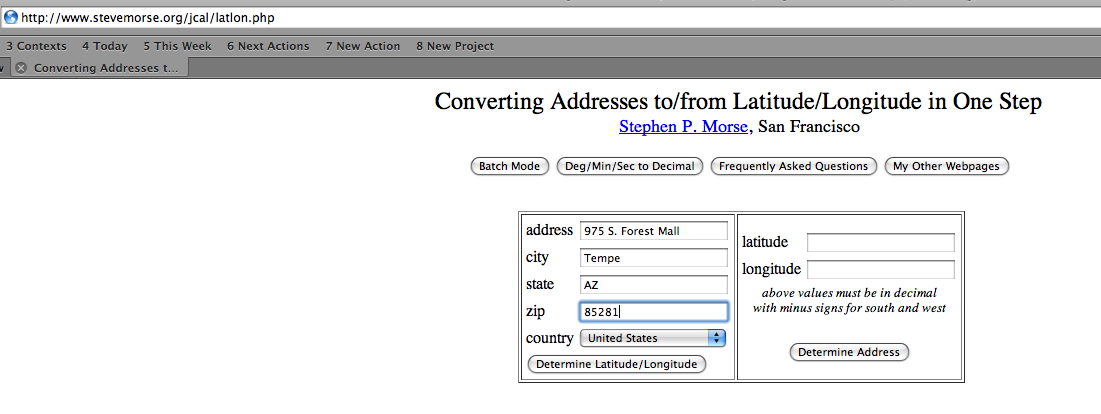
\includegraphics[width=.65\linewidth]{geocode1.png}
    \end{center}
 \end{frame} 

\begin{frame}
	\frametitle{Where is the office?}
    \begin{center}
      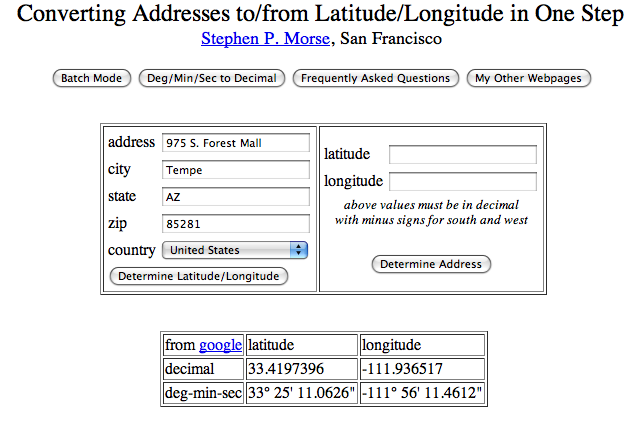
\includegraphics[width=.65\linewidth]{geocode2.png}
    \end{center}
 \end{frame} 

\begin{frame}
	\frametitle{Geocoding: google link}
    \begin{center}
      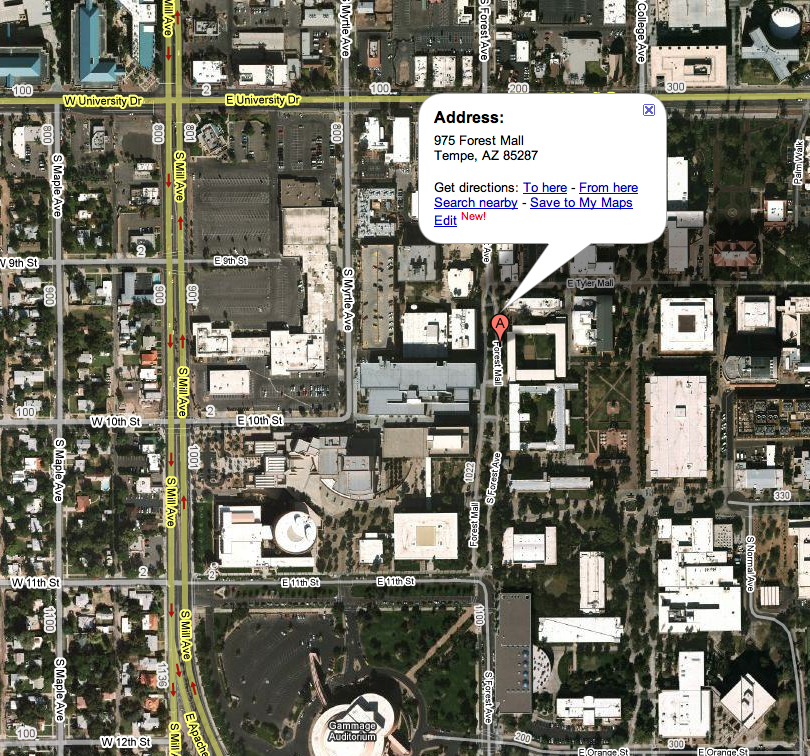
\includegraphics[width=.65\linewidth]{geocode3.png}
    \end{center}
 \end{frame} 

\begin{frame}
	\frametitle{Geocoding}
    \begin{center}
      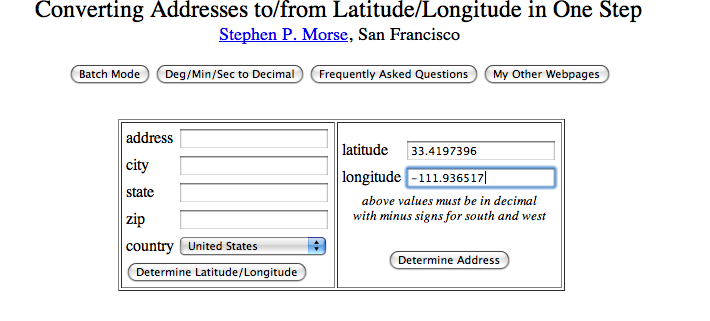
\includegraphics[width=.65\linewidth]{geocode4.png}
    \end{center}
 \end{frame} 

\begin{frame}
	\frametitle{Geocoding}
    \begin{center}
      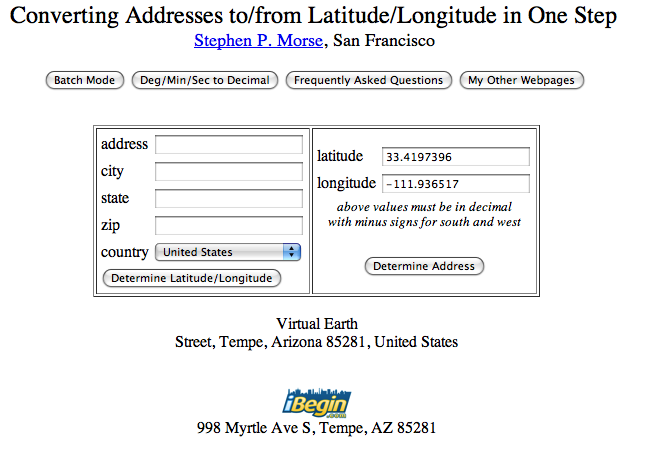
\includegraphics[width=.65\linewidth]{geocode5.png}
    \end{center}
 \end{frame} 

\begin{frame}
	\frametitle{Location}
 
\begin{block}{Location as a \alert{Given}}
 \begin{itemize}
 \item  in most spatial data analyses no choice in location
 \item  no sampling in the usual sense
 \item  data = attributes augmented with \alert{locational} information
 \end{itemize}
 \end{block} \end{frame} 

 \subsection{Spatial Effects}

\begin{frame}
	\frametitle{Spatial Effects}
 
\begin{block}{The Trilogy}
 \begin{itemize}
 \item Spatial Dependence
 \item Spatial Heterogeneity
 \item Spatial Scale
 \end{itemize}
 \end{block} \end{frame} 

\begin{frame}
	\frametitle{First Law of Geography}
 
\begin{block}{Waldo Tobler}
 \begin{itemize}
 \item	"everything depends on everything else, but closer things more so"
 \item	Structure of spatial dependence
 \item	Distance Decay
 \item	Closeness = Similarity
 \end{itemize}
 \end{block} \end{frame} 


\begin{frame}
  \frametitle{Spatial Heterogeneity}
  \begin{block}{Spatial Instability}
    \begin{itemize}
      \item Process varies in some way over spatial units
      \item Multiple forms
	\begin{itemize}
	  \item Discrete = regimes
	  \item Continuous = expansion method, GWR
	\end{itemize}
      \item Trade-off
	\begin{itemize}
	  \item spatial homogeneity = stationary process
	  \item uniqueness = extreme heterogeneity
	\end{itemize}
    \end{itemize}
   \end{block}
 \end{frame}

 \begin{frame}
   \frametitle{Spatial Scale}
   \begin{block}{Mismatch}
     \begin{itemize}
       \item Spatial scale of the process
       \item Spatial scale of our measurement
     \end{itemize}
    \end{block}
\begin{block}{Issues}
     \begin{itemize}
       \item points too far apart = miss small distance variation
       \item area aggregates cannot provide information on individual
	 behavior
       \item ecological fallacy
     \end{itemize}
    \end{block}

  \end{frame}
 
  \begin{frame}
    \frametitle{Modifiable Areal Unit Problem (MAUP)}
    \begin{block}{Aggregation Problem}
      \begin{itemize}
	\item special case of ecological fallacy
	\item spatial heterogeneity
	\item a million spatial autocorrelation coefficients
      \end{itemize}
    \end{block}
    \begin{block}{Zonation Problem}
      \begin{itemize}
	\item size
	\item arrangement
      \end{itemize}
    \end{block}
  \end{frame}
  \begin{frame}
    \frametitle{Spatial Heterogeneity: Housing Prices}
    \begin{center}
      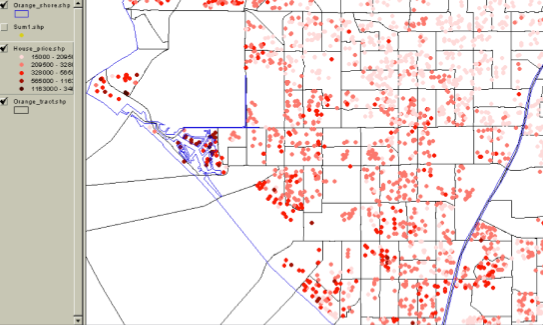
\includegraphics[width=.65\linewidth]{ochousing.png}
    \end{center}
  \end{frame}

  \begin{frame}
    \frametitle{Spatial Effects}
    \begin{block}{Dependence, Heterogeneity and Scale}
      \begin{itemize}
	\item not necessarily orthogonal
	\item distinguishing between dependence and heterogeneity can be
	  challenging
      \end{itemize}
     \end{block}
   \end{frame}

   \begin{frame}
     \frametitle{Spatial Sampling}
     \begin{block}{Location as an Experimental Design Problem}
       \begin{itemize}
	 \item Spatial sampling = where to collect the data
	   \begin{itemize}
	     \item which villages to survey
	     \item where to locate air quality monitoring stations
	   \end{itemize}
       \end{itemize}
      \end{block}
    \end{frame}


    \begin{frame}
      \frametitle{Spatial Sampling}
      \begin{center}
	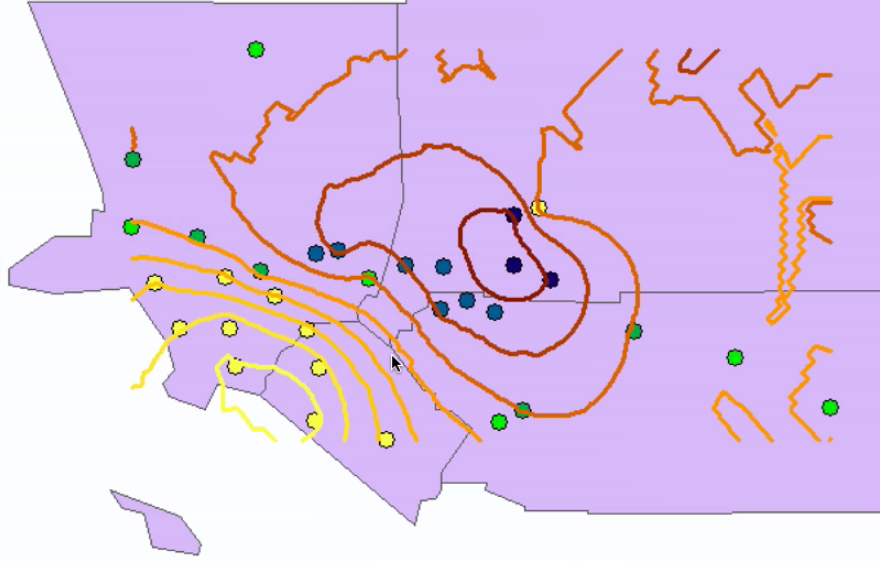
\includegraphics[width=.65\linewidth]{laozone.png}
      \end{center}
    \end{frame}

\section{Spatial Data Analysis} 
\subsection{Spatial Process}
\begin{frame}
  \frametitle{Spatial Process}
  \begin{block}{Spatial Random Field}
    \begin{itemize}
      \item a mathematical construct to capture randomness of values
	distributed over space
      \item $ \{ Z(s):s \in D \} $
	\begin{itemize}
	  \item $s \in R^d:$ location (e.g., lat-lon)
	  \item $D \in R^d:$ index set = possible locations
	  \item $Z(s):$ random variable at location $s$
	\end{itemize}
    \end{itemize}
   \end{block}
 \end{frame}
 \begin{frame}
   \frametitle{Types of Spatial Analysis}
   \begin{block}{Point Pattern Analysis}
      spatial distribution of events
    \end{block}
   \begin{block}{Geostatistical Analysis}
      surface modeling
    \end{block}
   \begin{block}{Lattice Data Analysis}
     spatial patterns of attributes observed for spatial objects
    \end{block}
  \end{frame}
  \subsection{Point Pattern Analysis}
  \begin{frame}
    \frametitle{Point Pattern Analysis}
    \begin{block}{Data}
      \begin{itemize}
	\item mapped pattern = all the events
	\item not a sample in the usual sense
      \end{itemize}
     \end{block}
    \begin{block}{Spatial Process}
      \begin{itemize}
	\item observations as a realization of a random point process
	\item points occur in space according to a mathematical model 
      \end{itemize}
     \end{block}
   \end{frame}
   \begin{frame}
     \frametitle{Point Data}
     \begin{block}{Spatial Domain: $D$}
       \begin{itemize}
	 \item Domain is \emph{random}
	 \item \emph{Number} of points is \emph{random}
	 \item \emph{Location} of points is \emph{random}
       \end{itemize}
      \end{block}
      \begin{block}{Focus: Properties of $D$}
	\begin{itemize}
	  \item Number of points observed
	  \item Pattern of the point locations
	\end{itemize}
      \end{block}
    \end{frame}


    \begin{frame}
      \frametitle{Point Patterns}
      \begin{center}
	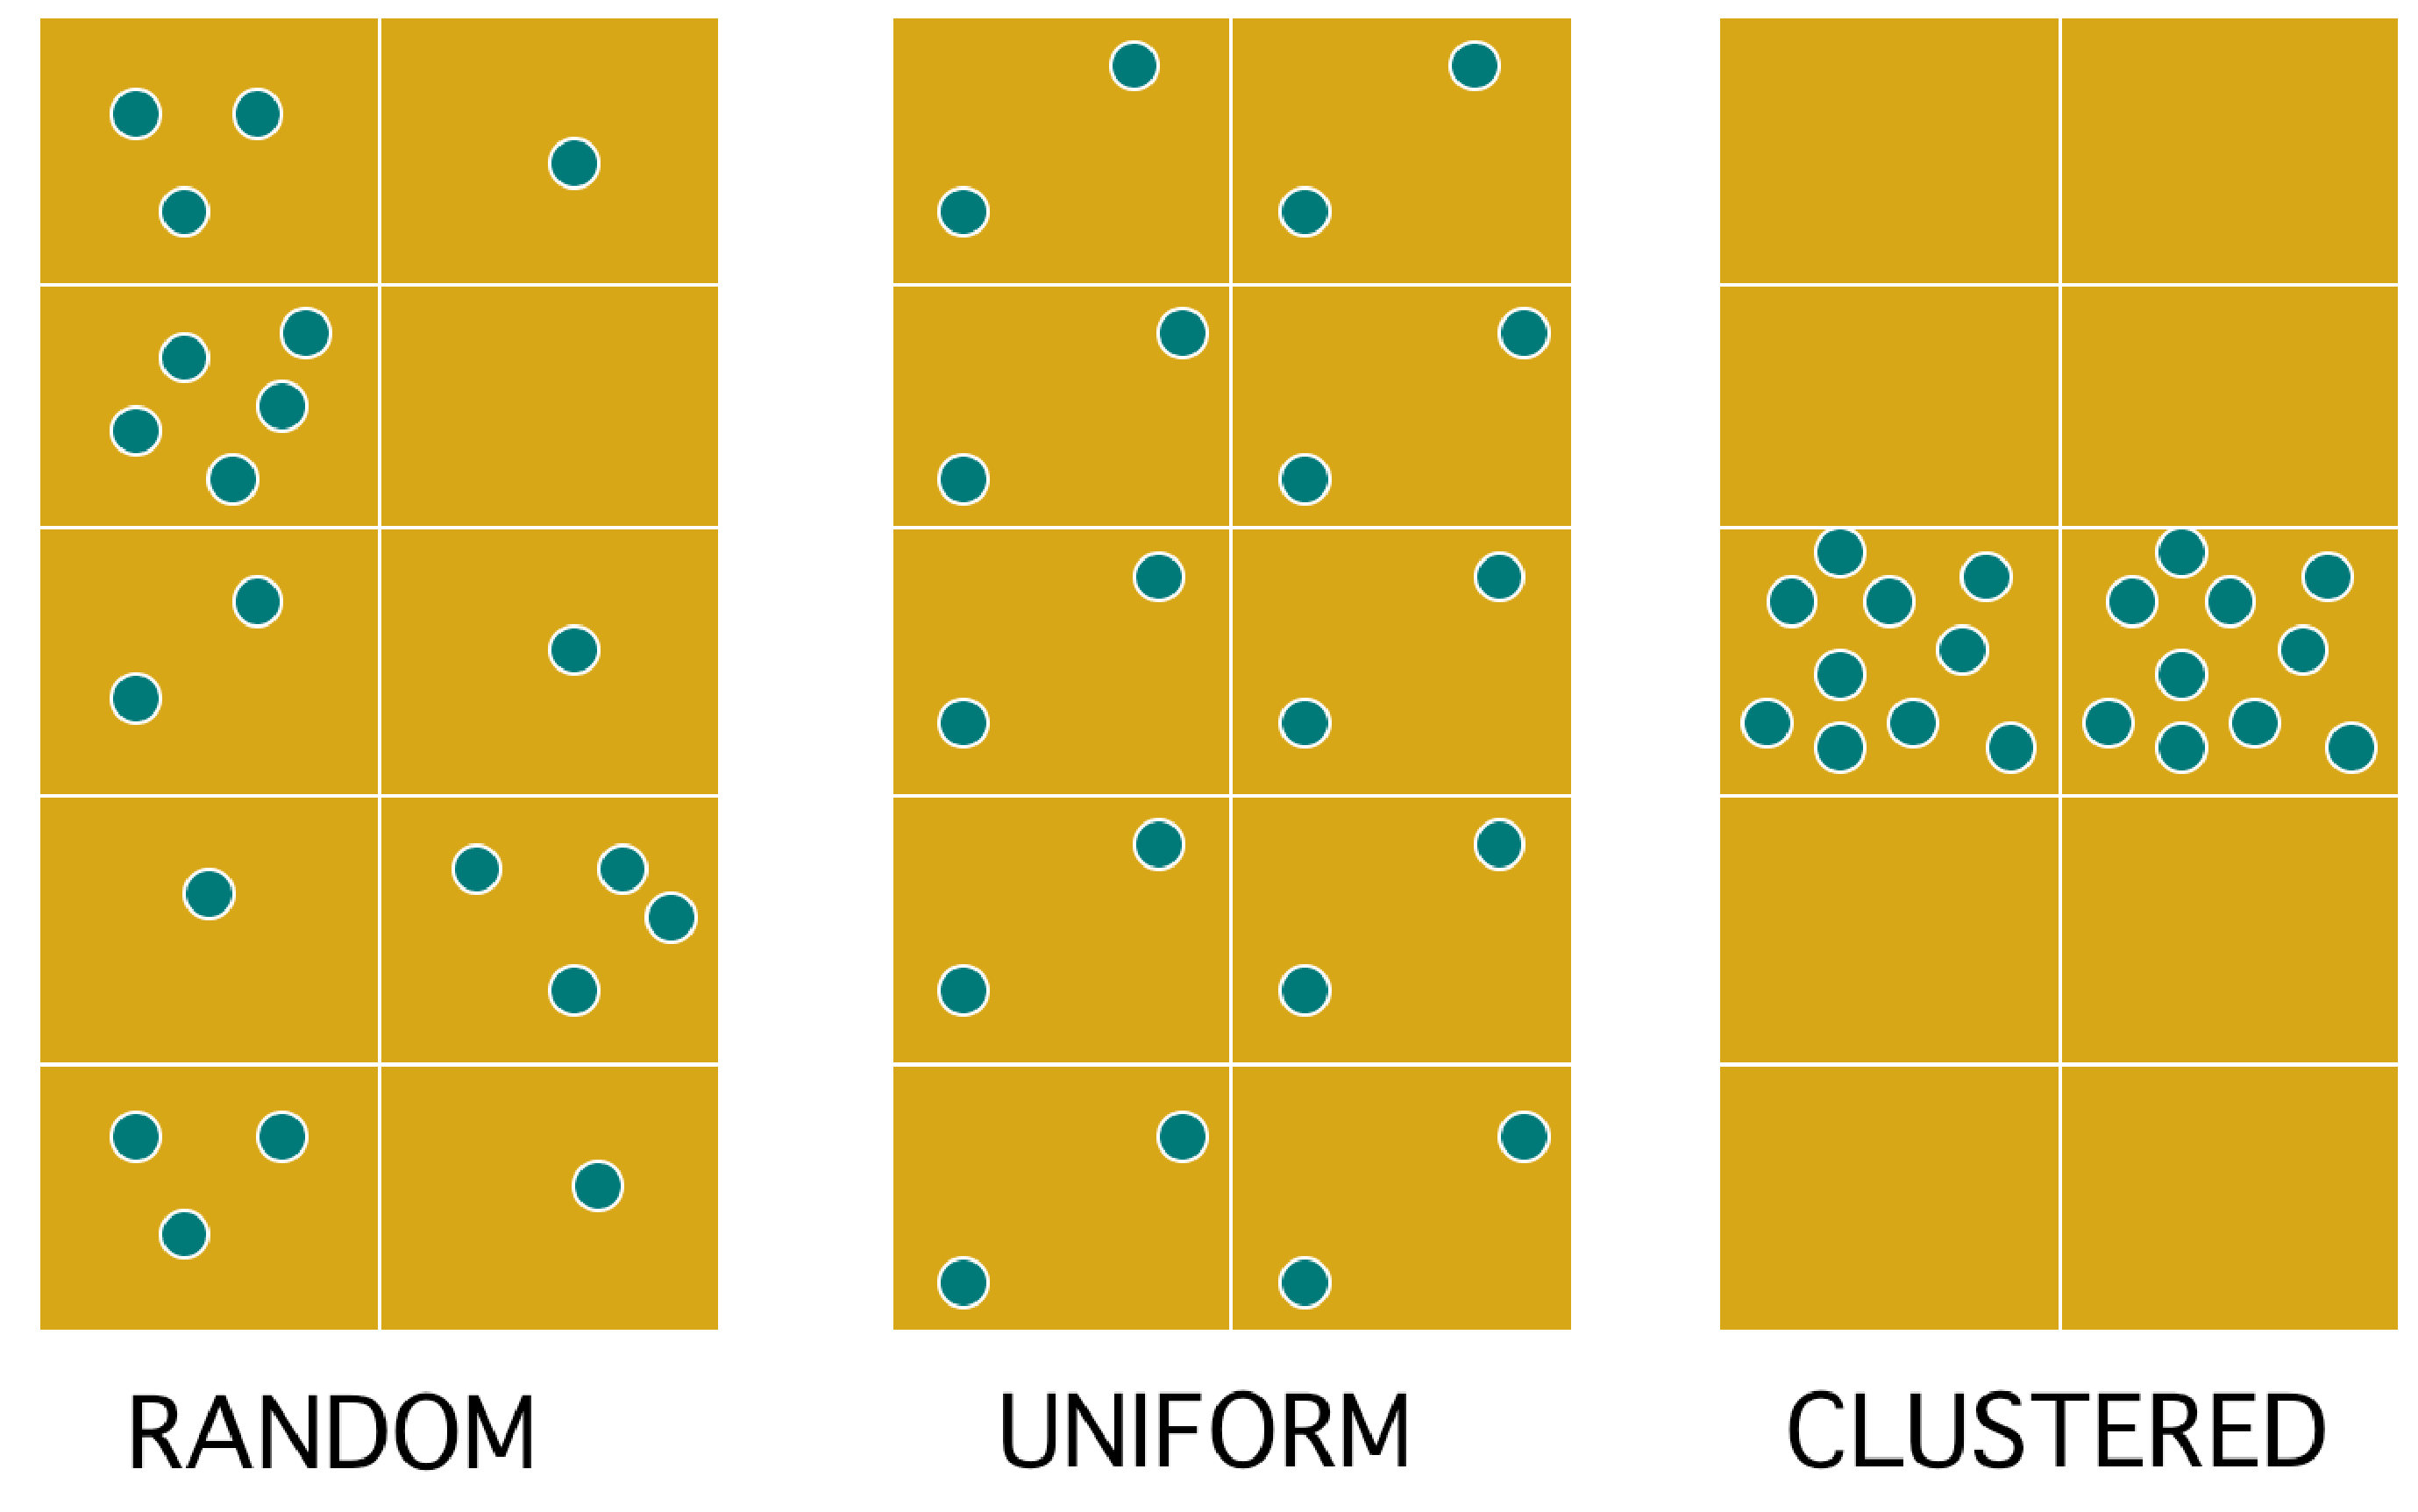
\includegraphics[width=.65\linewidth]{pointtypes.pdf}
      \end{center}
    \end{frame}
    \begin{frame}
      \frametitle{Point Patterns}
      \begin{block}{Unmarked Point Pattern}
	\begin{itemize}
	  \item Only location is recorded
	  \item No other attribute information
	\end{itemize}
      \end{block}
      \begin{block}{Marked Point Patterns}
	\begin{itemize}
	  \item Location is recorded
	  \item Stochastic attributes also recorded
	  \item e.g., sales at location, dbh of tree
	\end{itemize}
      \end{block}
    \end{frame}

    \begin{frame}
       \frametitle{Point Pattern Analysis: Quadrat Methods}
       \begin{center}
	 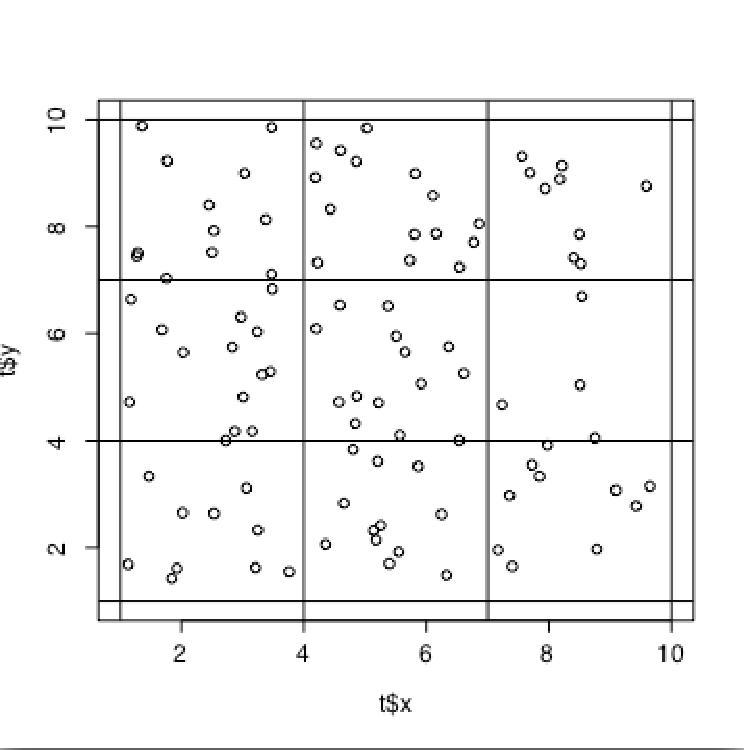
\includegraphics[width=.65\linewidth]{plotquad.pdf}
       \end{center}
     \end{frame}

     \begin{frame}
       \frametitle{Point Pattern Analysis: Distance Based Methods}
       \begin{center}
	 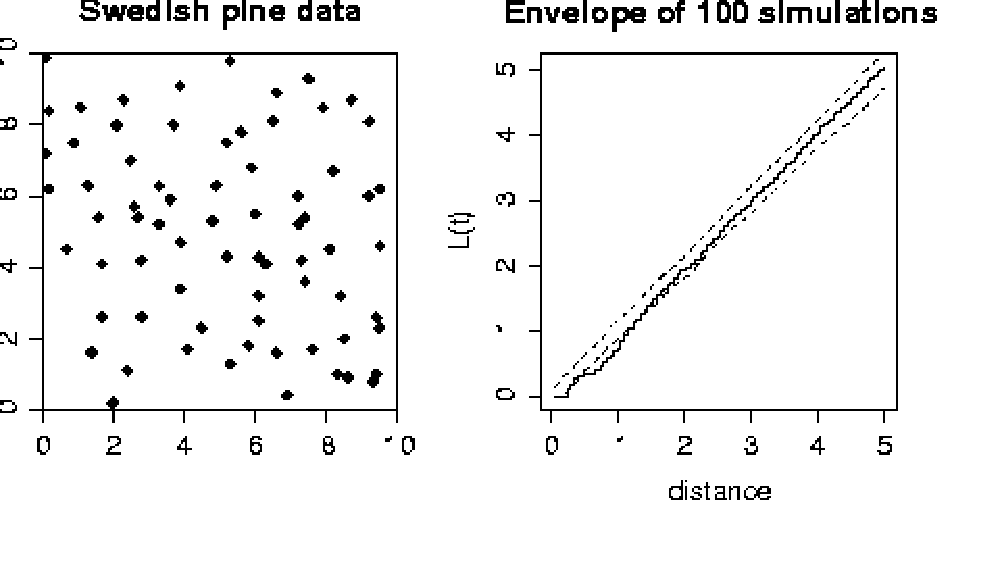
\includegraphics[width=.65\linewidth]{pinepoint.pdf}
       \end{center}
     \end{frame}

     \begin{frame}
       \frametitle{Points on Networks}
       \begin{center}
	 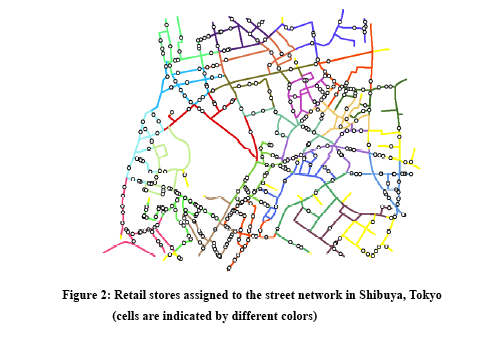
\includegraphics[width=.65\linewidth]{sanet.jpg}
       \end{center}
     \end{frame}

     \begin{frame}
       \frametitle{Burkitt's Lymphoma Data: Time Series of Point Data}
       \begin{center}
	 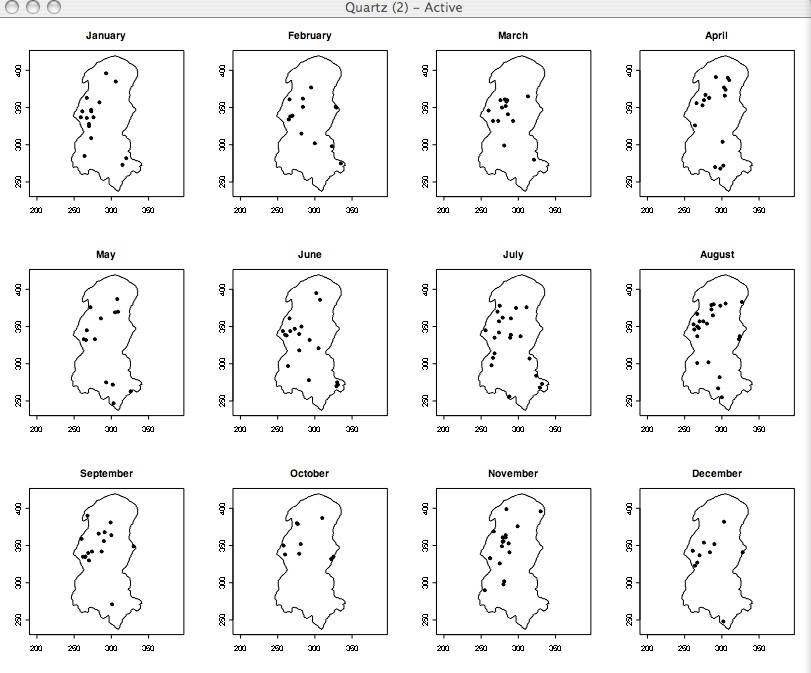
\includegraphics[width=.65\linewidth]{tspoints.jpg}
       \end{center}
     \end{frame}


\subsection{Lattice}
\begin{frame}[<+->]
  \frametitle{Lattice Data}
  \begin{block}{Spatial Domain: $D$ }
    \begin{itemize}
      \item Discrete and fixed
      \item Locations nonrandom
      \item Locations countable
    \end{itemize}
   \end{block}
\begin{block}{Examples of lattice data}
    \begin{itemize}
      \item Attributes collected by ZIP code
      \item census tract
      \item remotely sensed data reported by pixels
    \end{itemize}
   \end{block}
 \end{frame}
\begin{frame}[<+->]
  \frametitle{Lattice Data: Indexing}
  \begin{block}{Site }
    \begin{itemize}
      \item Each location is now an area or \emph{site}
      \item One observation on $Z$ for each site
      \item Need a spatial index: $Z(s_i)$
    \end{itemize}
   \end{block}
\begin{block}{$Z(s_i)$}
    \begin{itemize}
      \item $s_i$ is a representative location within the site
      \item e.g., centroid, largest city
      \item Allows for measuring distances between sites
    \end{itemize}
   \end{block}
 \end{frame}
\begin{frame}[<+->]
  \frametitle{Lattice Data: Aggregation and Coverage}
  \begin{block}{Sites are areal units}
    \begin{itemize}
      \item Attribute is typically aggregated or averaged
      \item Aggregated: event counts (number of crimes per tract)
      \item Averaged: per capita income by state
    \end{itemize}
   \end{block}
\begin{block}{Coverage}
    \begin{itemize}
      \item Lattice data is usually exhaustive in coverage
      \item e.g., U.S. states, census tracts in San Diego
      \item Prediction or interpolation not meaningful
      \item Explaining attribute variation across sites is the focus
    \end{itemize}
   \end{block}
 \end{frame}
\begin{frame}
    \frametitle{Lattice Data: State Per Capita Incomes}
    \begin{center}
      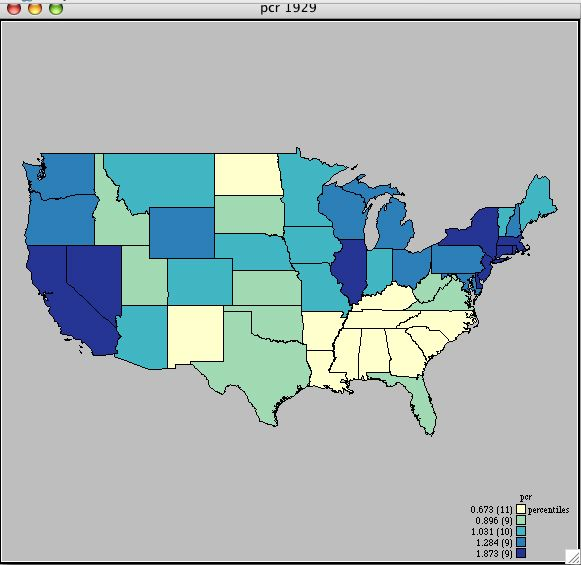
\includegraphics[width=.65\linewidth]{lattice}
    \end{center}
  \end{frame}
\begin{frame}
    \frametitle{Lattice Data: Spatial Autocorrelation}
    \begin{center}
      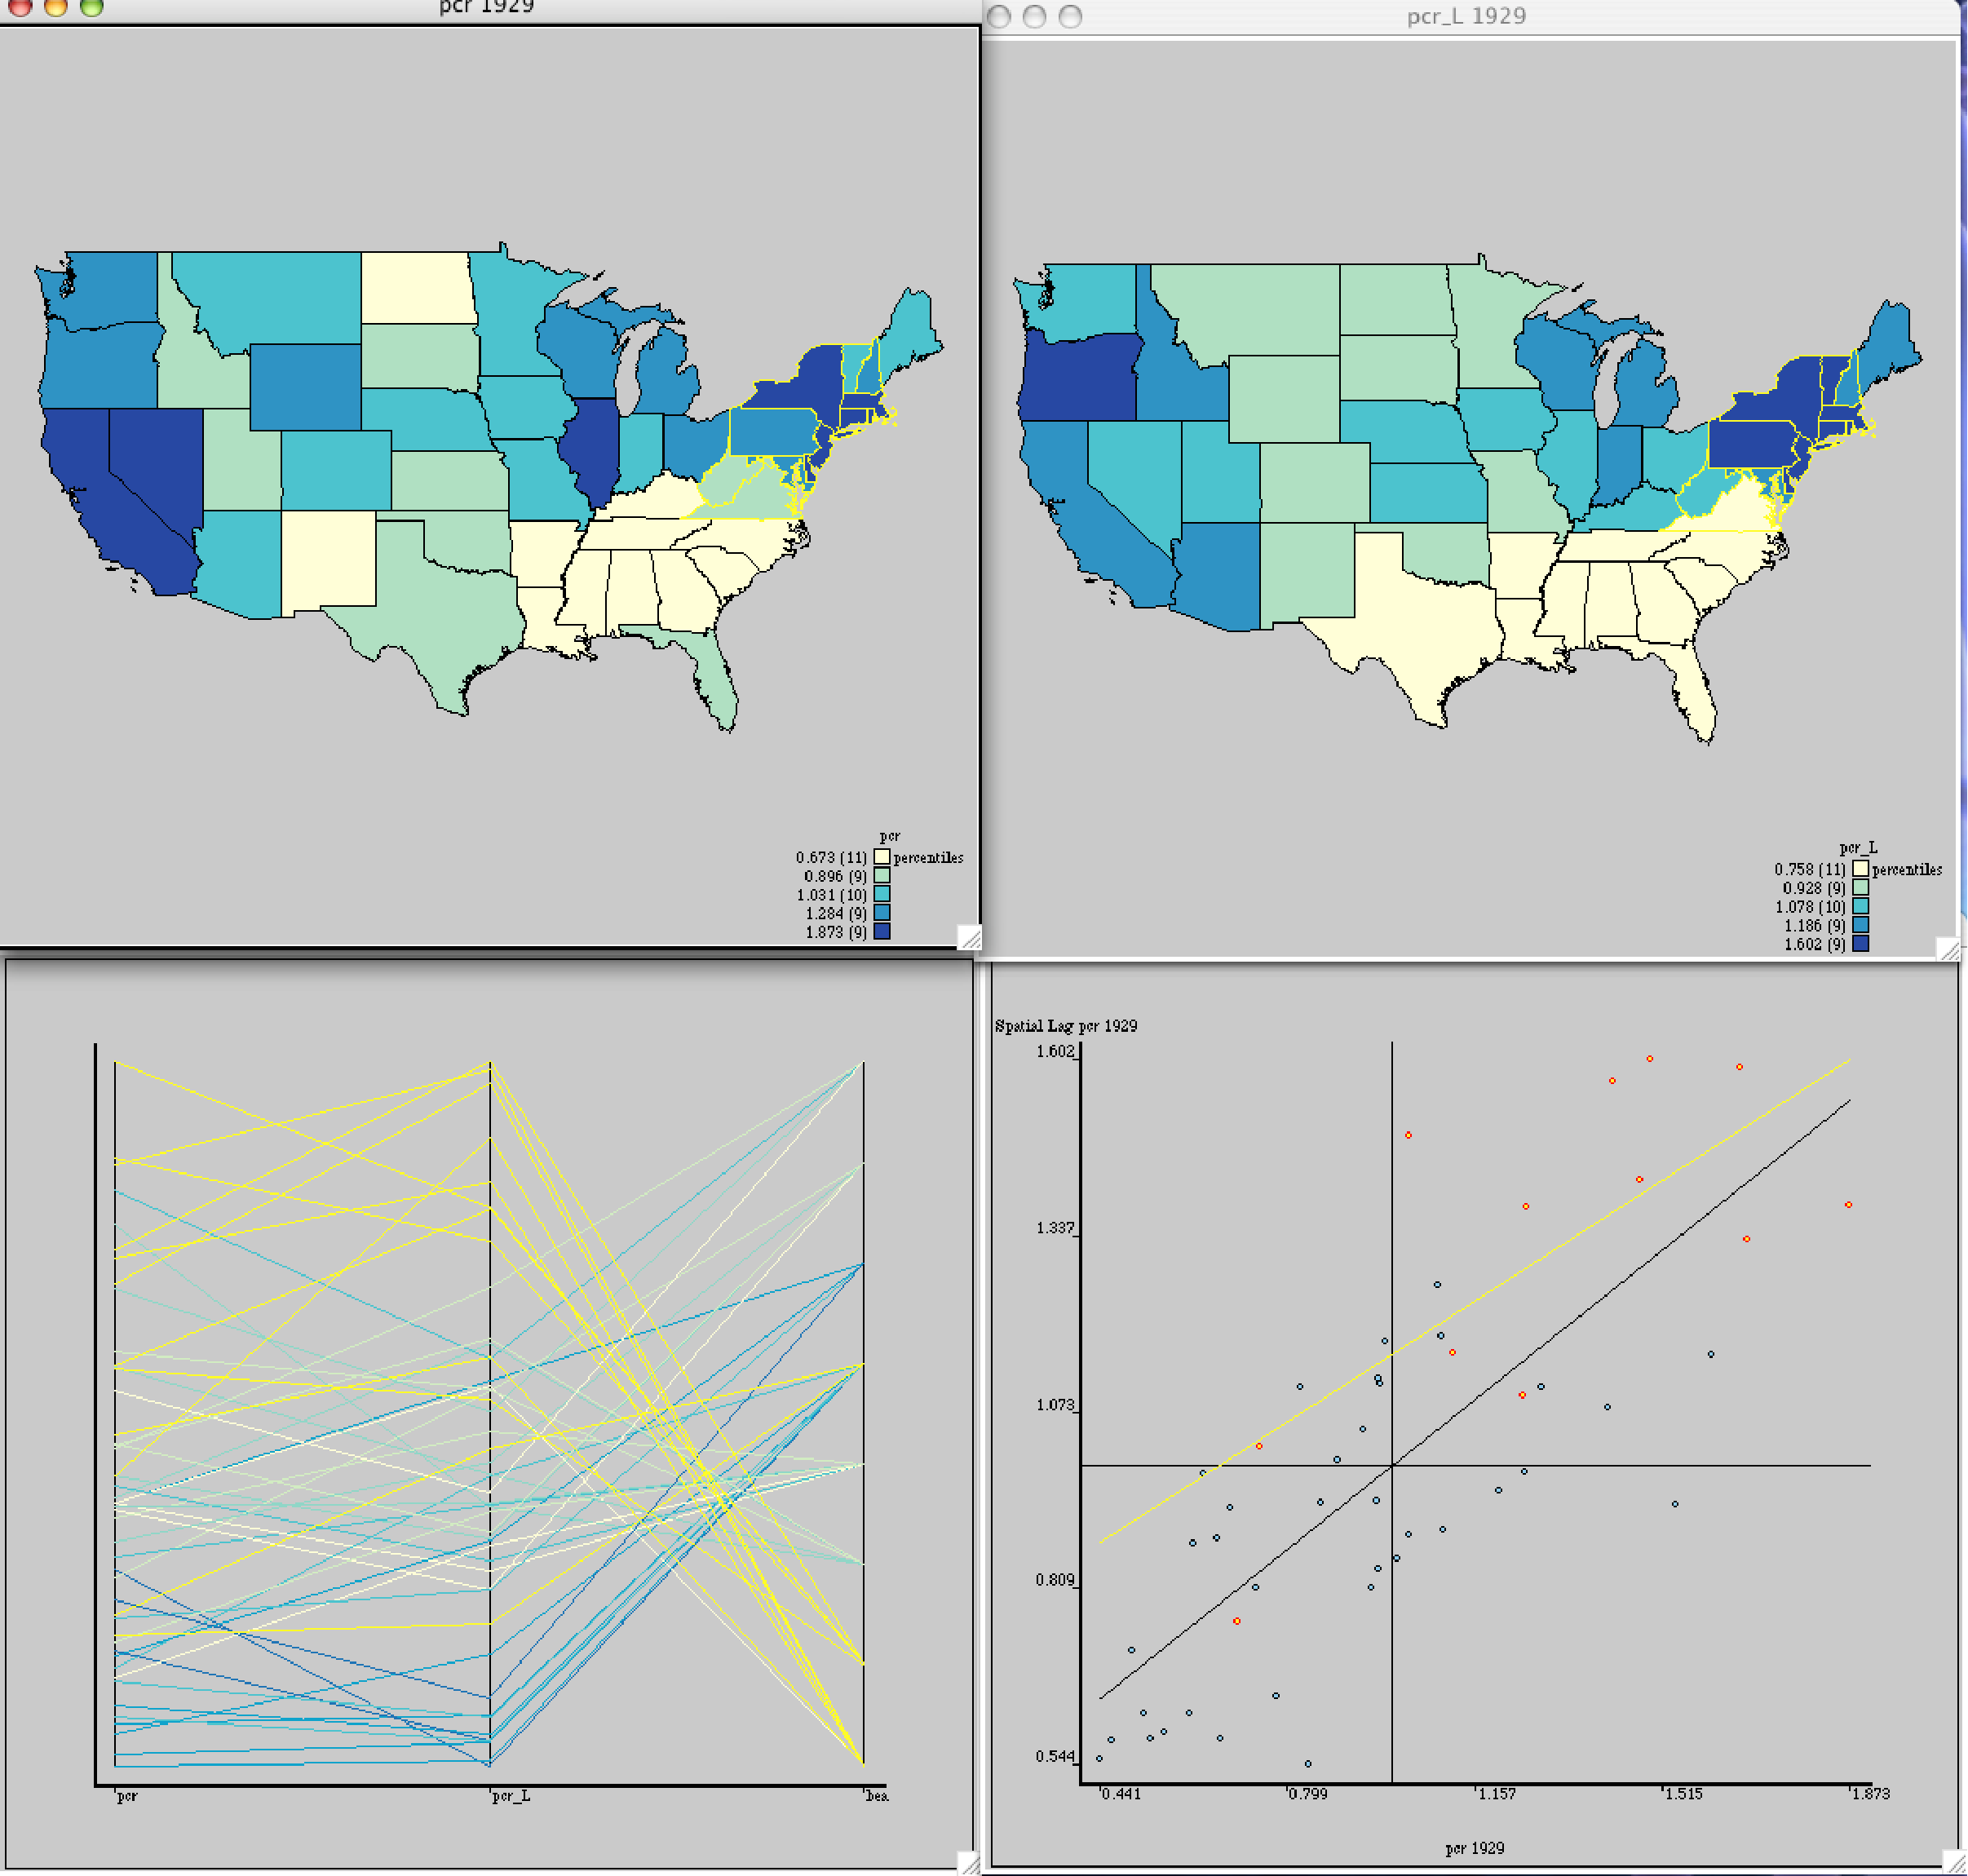
\includegraphics[width=.65\linewidth]{lattice2}
    \end{center}
  \end{frame}



\subsection{Geostatistical}
\begin{frame}[<+->]
  \frametitle{Geostatistical Data}
  \begin{block}{Spatial Domain: $D$ }
    \begin{itemize}
      \item A continuous and fixed set.
      \item Meaning $Z(s)$ can be observed everywhere within $D$.
      \item Between any two sample locations $s_i$ and $s_j$ you can
	theoretically place an infinite number of other samples.
      \item By fixed: the points in $D$ are non-stochastic
    \end{itemize}
   \end{block}
\begin{block}{Continuous Variation}
    \begin{itemize}
      \item Because of the continuity of $D$
      \item Geostatistical data is referred to as ``spatial data with
	continuous variation.''
      \item Continuity is associated with $D$.
      \item Attribute $Z$ may, or may not, be continuous.
    \end{itemize}
   \end{block}
 \end{frame}
 \begin{frame}
   \frametitle{Geostatistical Data: Rainfall in Parana State Brazil}
   \begin{center}
     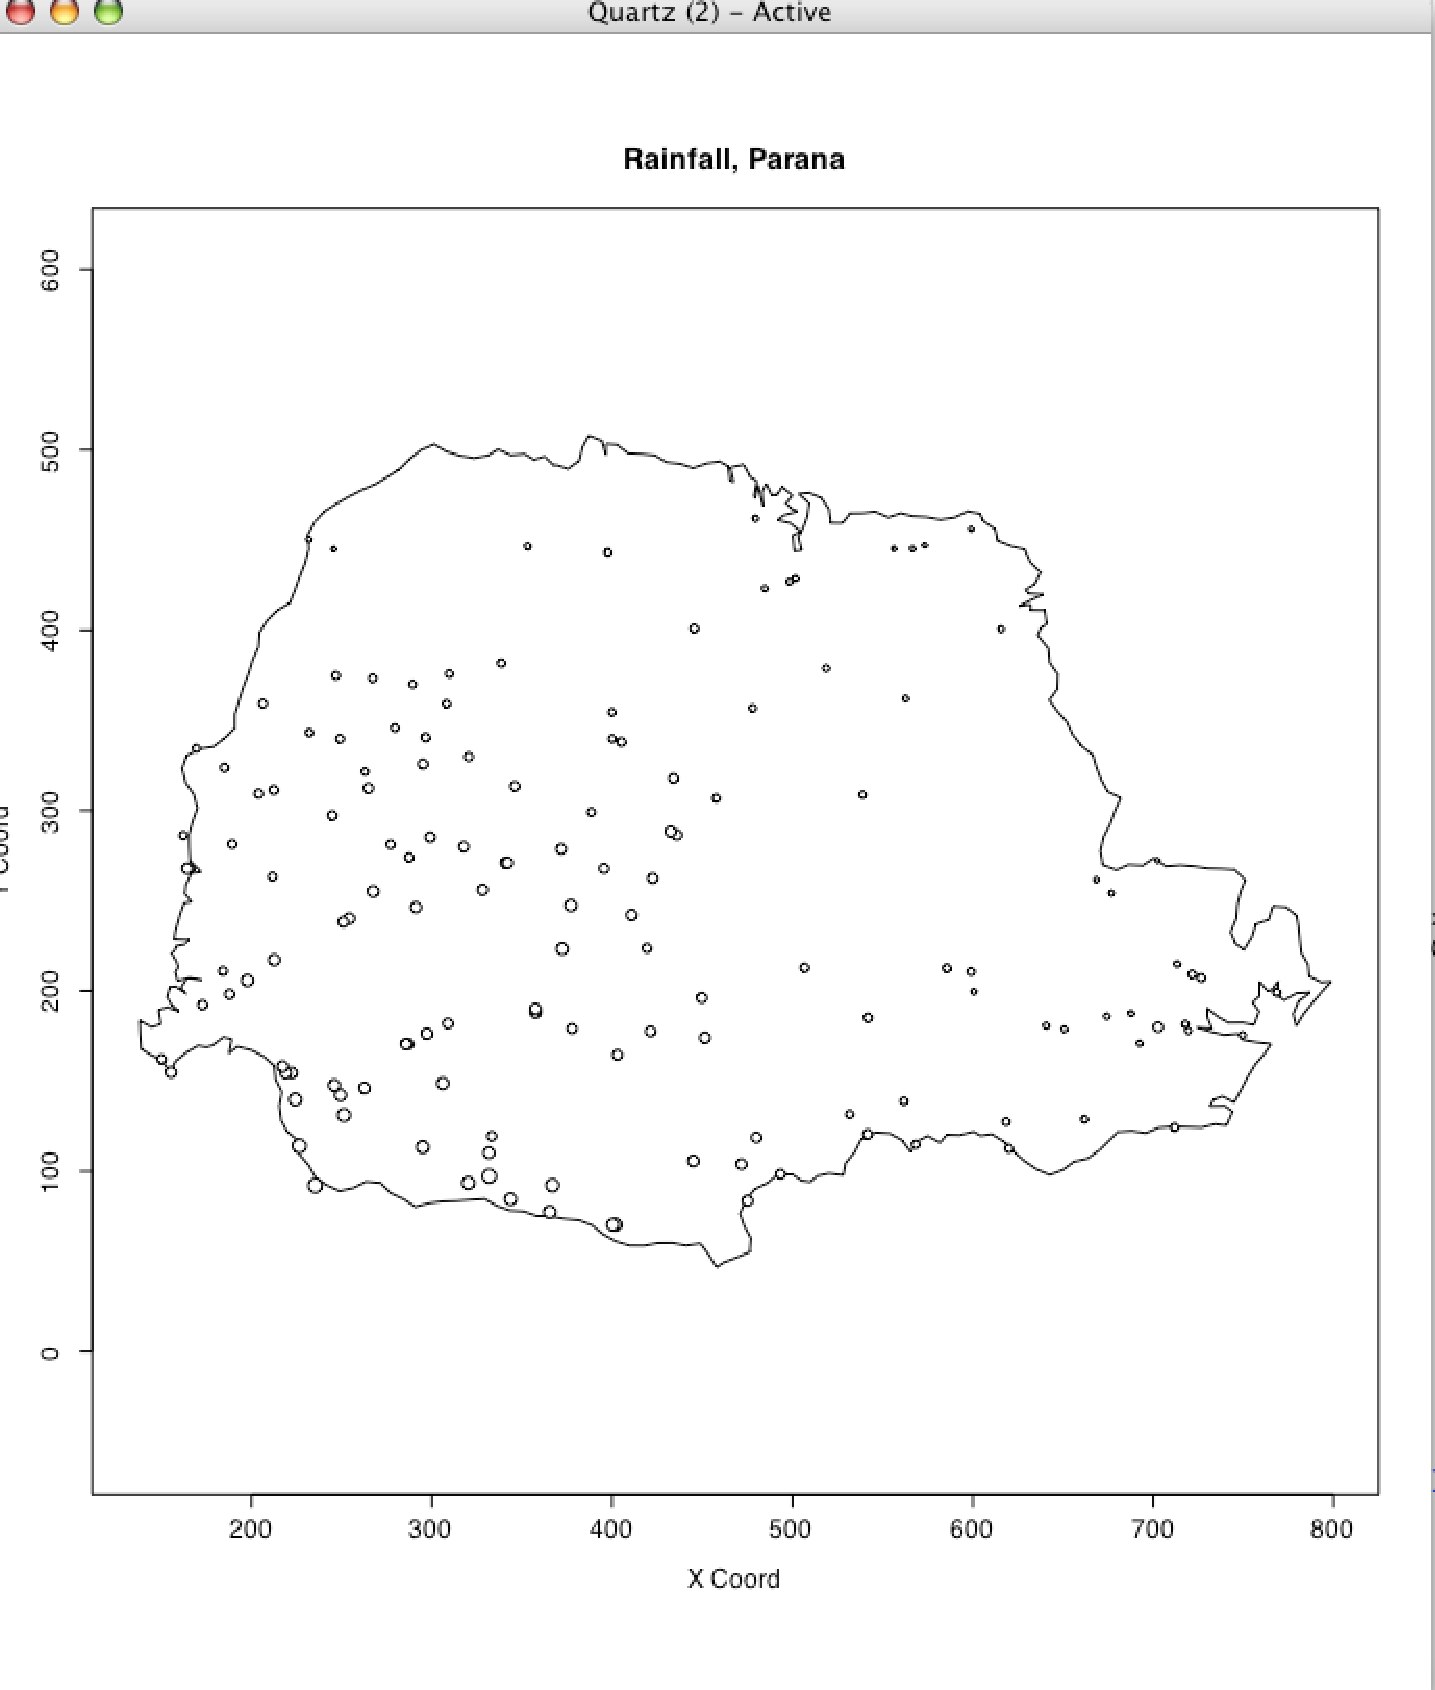
\includegraphics[width=.65\linewidth]{rainfall.pdf}
   \end{center}
 \end{frame}
 \begin{frame}[<+->]
   \frametitle{Geostatistical Data}
   \begin{block}{Continuous variation}
     \begin{itemize}
       \item Potentially measurable anywhere in $D$
       \item Impossible to sample $D$ exhaustively
     \end{itemize}
    \end{block}
\begin{block}{Reconstruction of the surface from observed sites}
     \begin{itemize}
       \item Tessellation based methods
       \item Interpolation
       \item Kriging
     \end{itemize}
    \end{block}
  \end{frame}
  \begin{frame}
    \frametitle{Surface Reconstruction: Example\footnote{From Goovaerts, P.
    (1999)``Performance comparison of geostatistical algorithms for
    incorporating elevation into the mapping of precipitation''.
    \emph{Geocomputation '99}.}}
    \begin{center}
      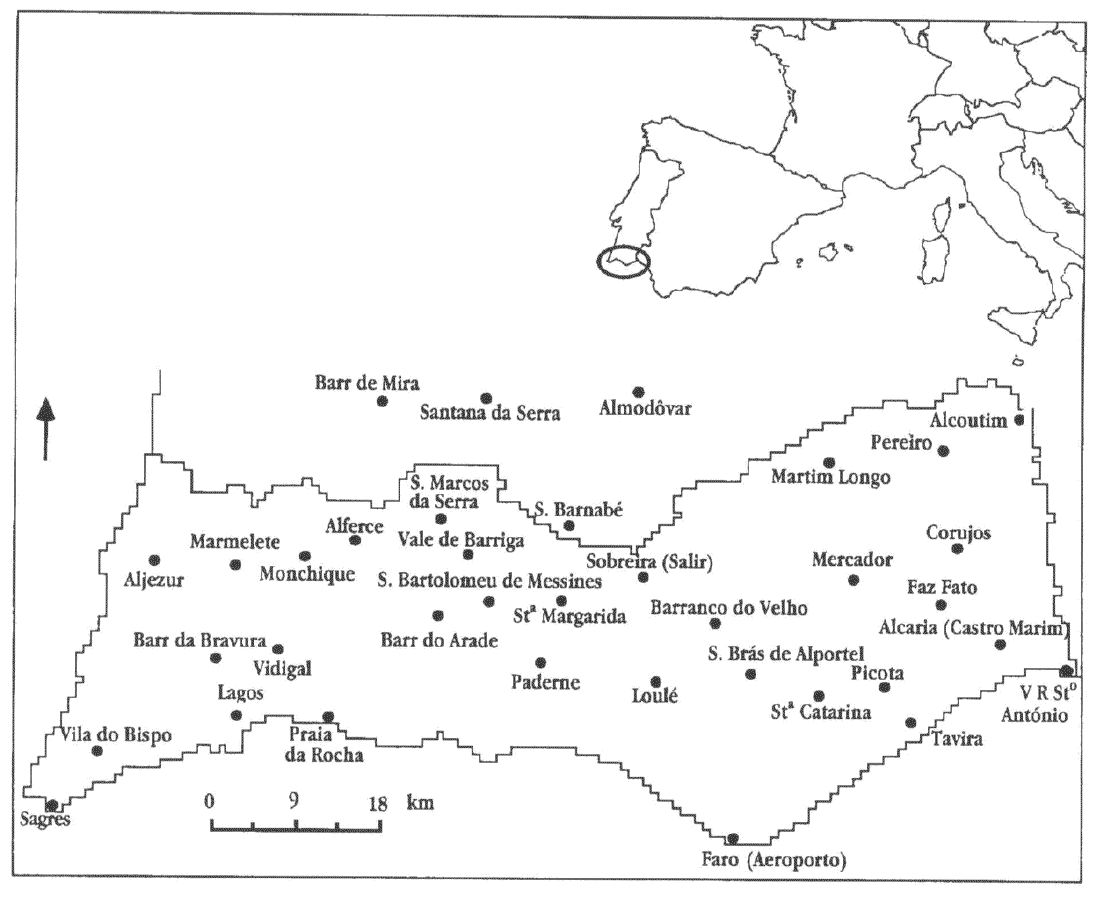
\includegraphics[width=.65\linewidth]{pg1.jpg}
    \end{center}
  \end{frame}
\begin{frame}
    \frametitle{Surface Reconstruction: Tessellation Based Method}
    \begin{center}
      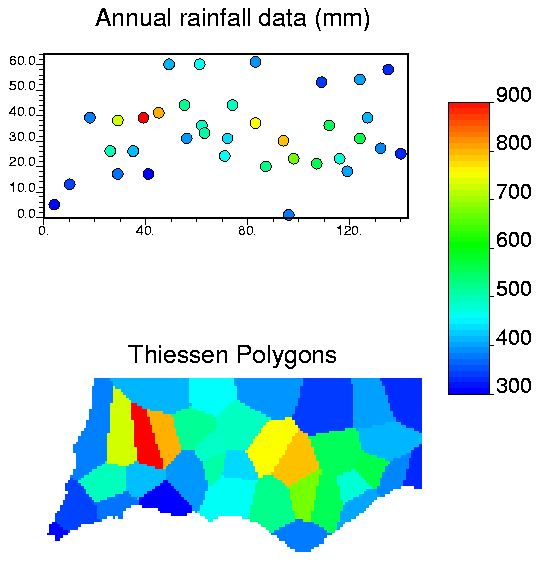
\includegraphics[width=.65\linewidth]{pg2.jpg}
    \end{center}
  \end{frame}
\begin{frame}
    \frametitle{Surface Reconstruction: Spatial Interpolation}
    \begin{center}
      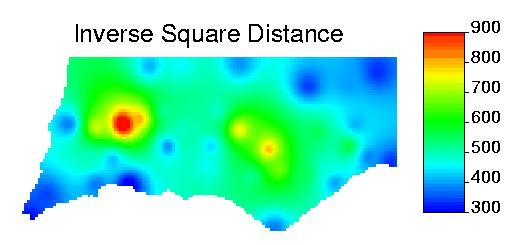
\includegraphics[width=.65\linewidth]{pg3.jpg}
    \end{center}
  \end{frame}
\begin{frame}
    \frametitle{Surface Reconstruction: Kriging}
    \begin{center}
      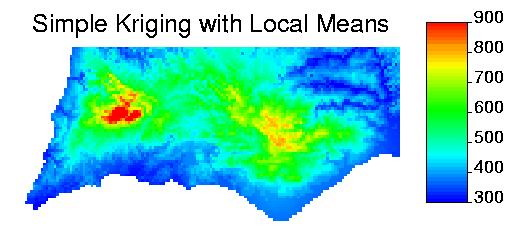
\includegraphics[width=.65\linewidth]{pg4.jpg}
    \end{center}
  \end{frame}




  \subsection{Network Data}
\begin{frame}[<+->]
  \frametitle{Network Data}
  \begin{block}{Networks} \begin{itemize} \item 	 A network is a system
      of linear features connected at intersections and interchanges.  \item
      These intersections and interchanges are called nodes.  \item 	The
      linear feature connecting any given pair of nodes is called an arc.
    \item 	Formally, a network is defined as a directed graph $G = (N,
      A)$ consisting of an indexed set of nodes $N$ with $n = |N|$ and a spanning
      set of directed arcs $A$ with $m = |A|$, where $n$ is the number of nodes and
      $m$ is the number of arcs.
  \item 	 Each arc on a network is represented as an ordered pair of
    nodes, in the form from node $i$ to node $j$, denoted by $(i, j)$.
  \item 	In the GIS literature, a network arc is often called a network link.
    \end{itemize}
   \end{block}
 \end{frame}

\begin{frame}
    \frametitle{Network Data: Graph Theory}
    \begin{center}
     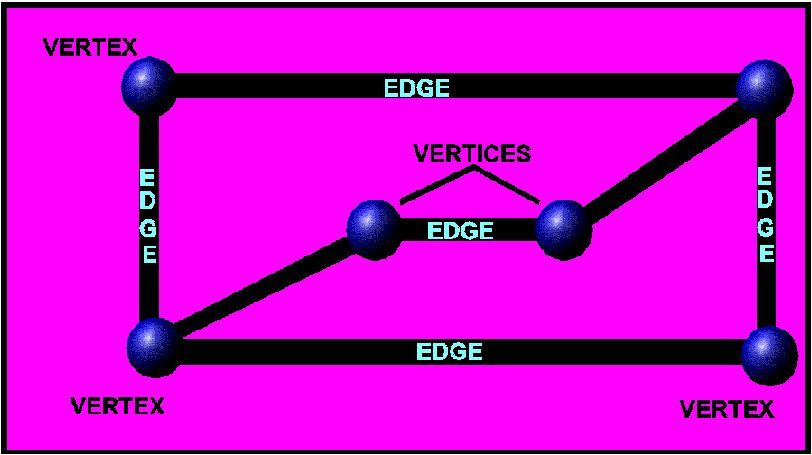
\includegraphics[width=.65\linewidth]{graph.jpg}
   \end{center}
\end{frame}

\begin{frame}[<+->]
    \frametitle{Network Data}
	\begin{block}{In this course}
  \begin{itemize}
	    \item We will not be analyzing network data per se
	    \item We will be drawing on graph theory to help in ESDA
	  \end{itemize}
	\end{block}
	\begin{block}{Uses of graph theory in ESDA}
	  \begin{itemize}
	    \item Properties of adjacency matrices
	    \item Clustering and regionalization algorithms
	  \end{itemize}
	 \end{block}
  \end{frame}

\begin{frame}
    \frametitle{Network Data: Adjacency Matrices}
    \begin{center}
      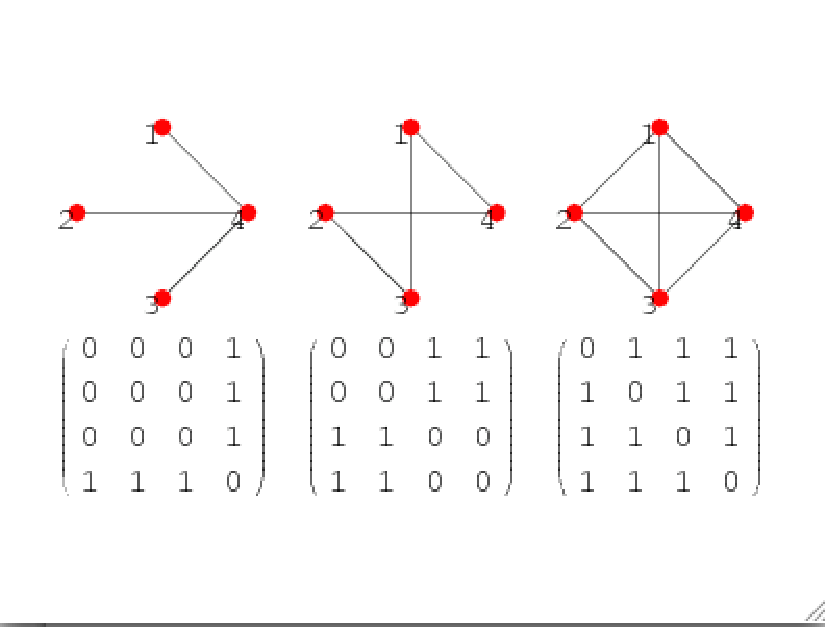
\includegraphics[width=.65\linewidth]{AdjacencyMatrix.pdf}
    \end{center}
  \end{frame}


\begin{frame}
    \frametitle{Network Data: Clustering Visualization}
    \begin{center}
      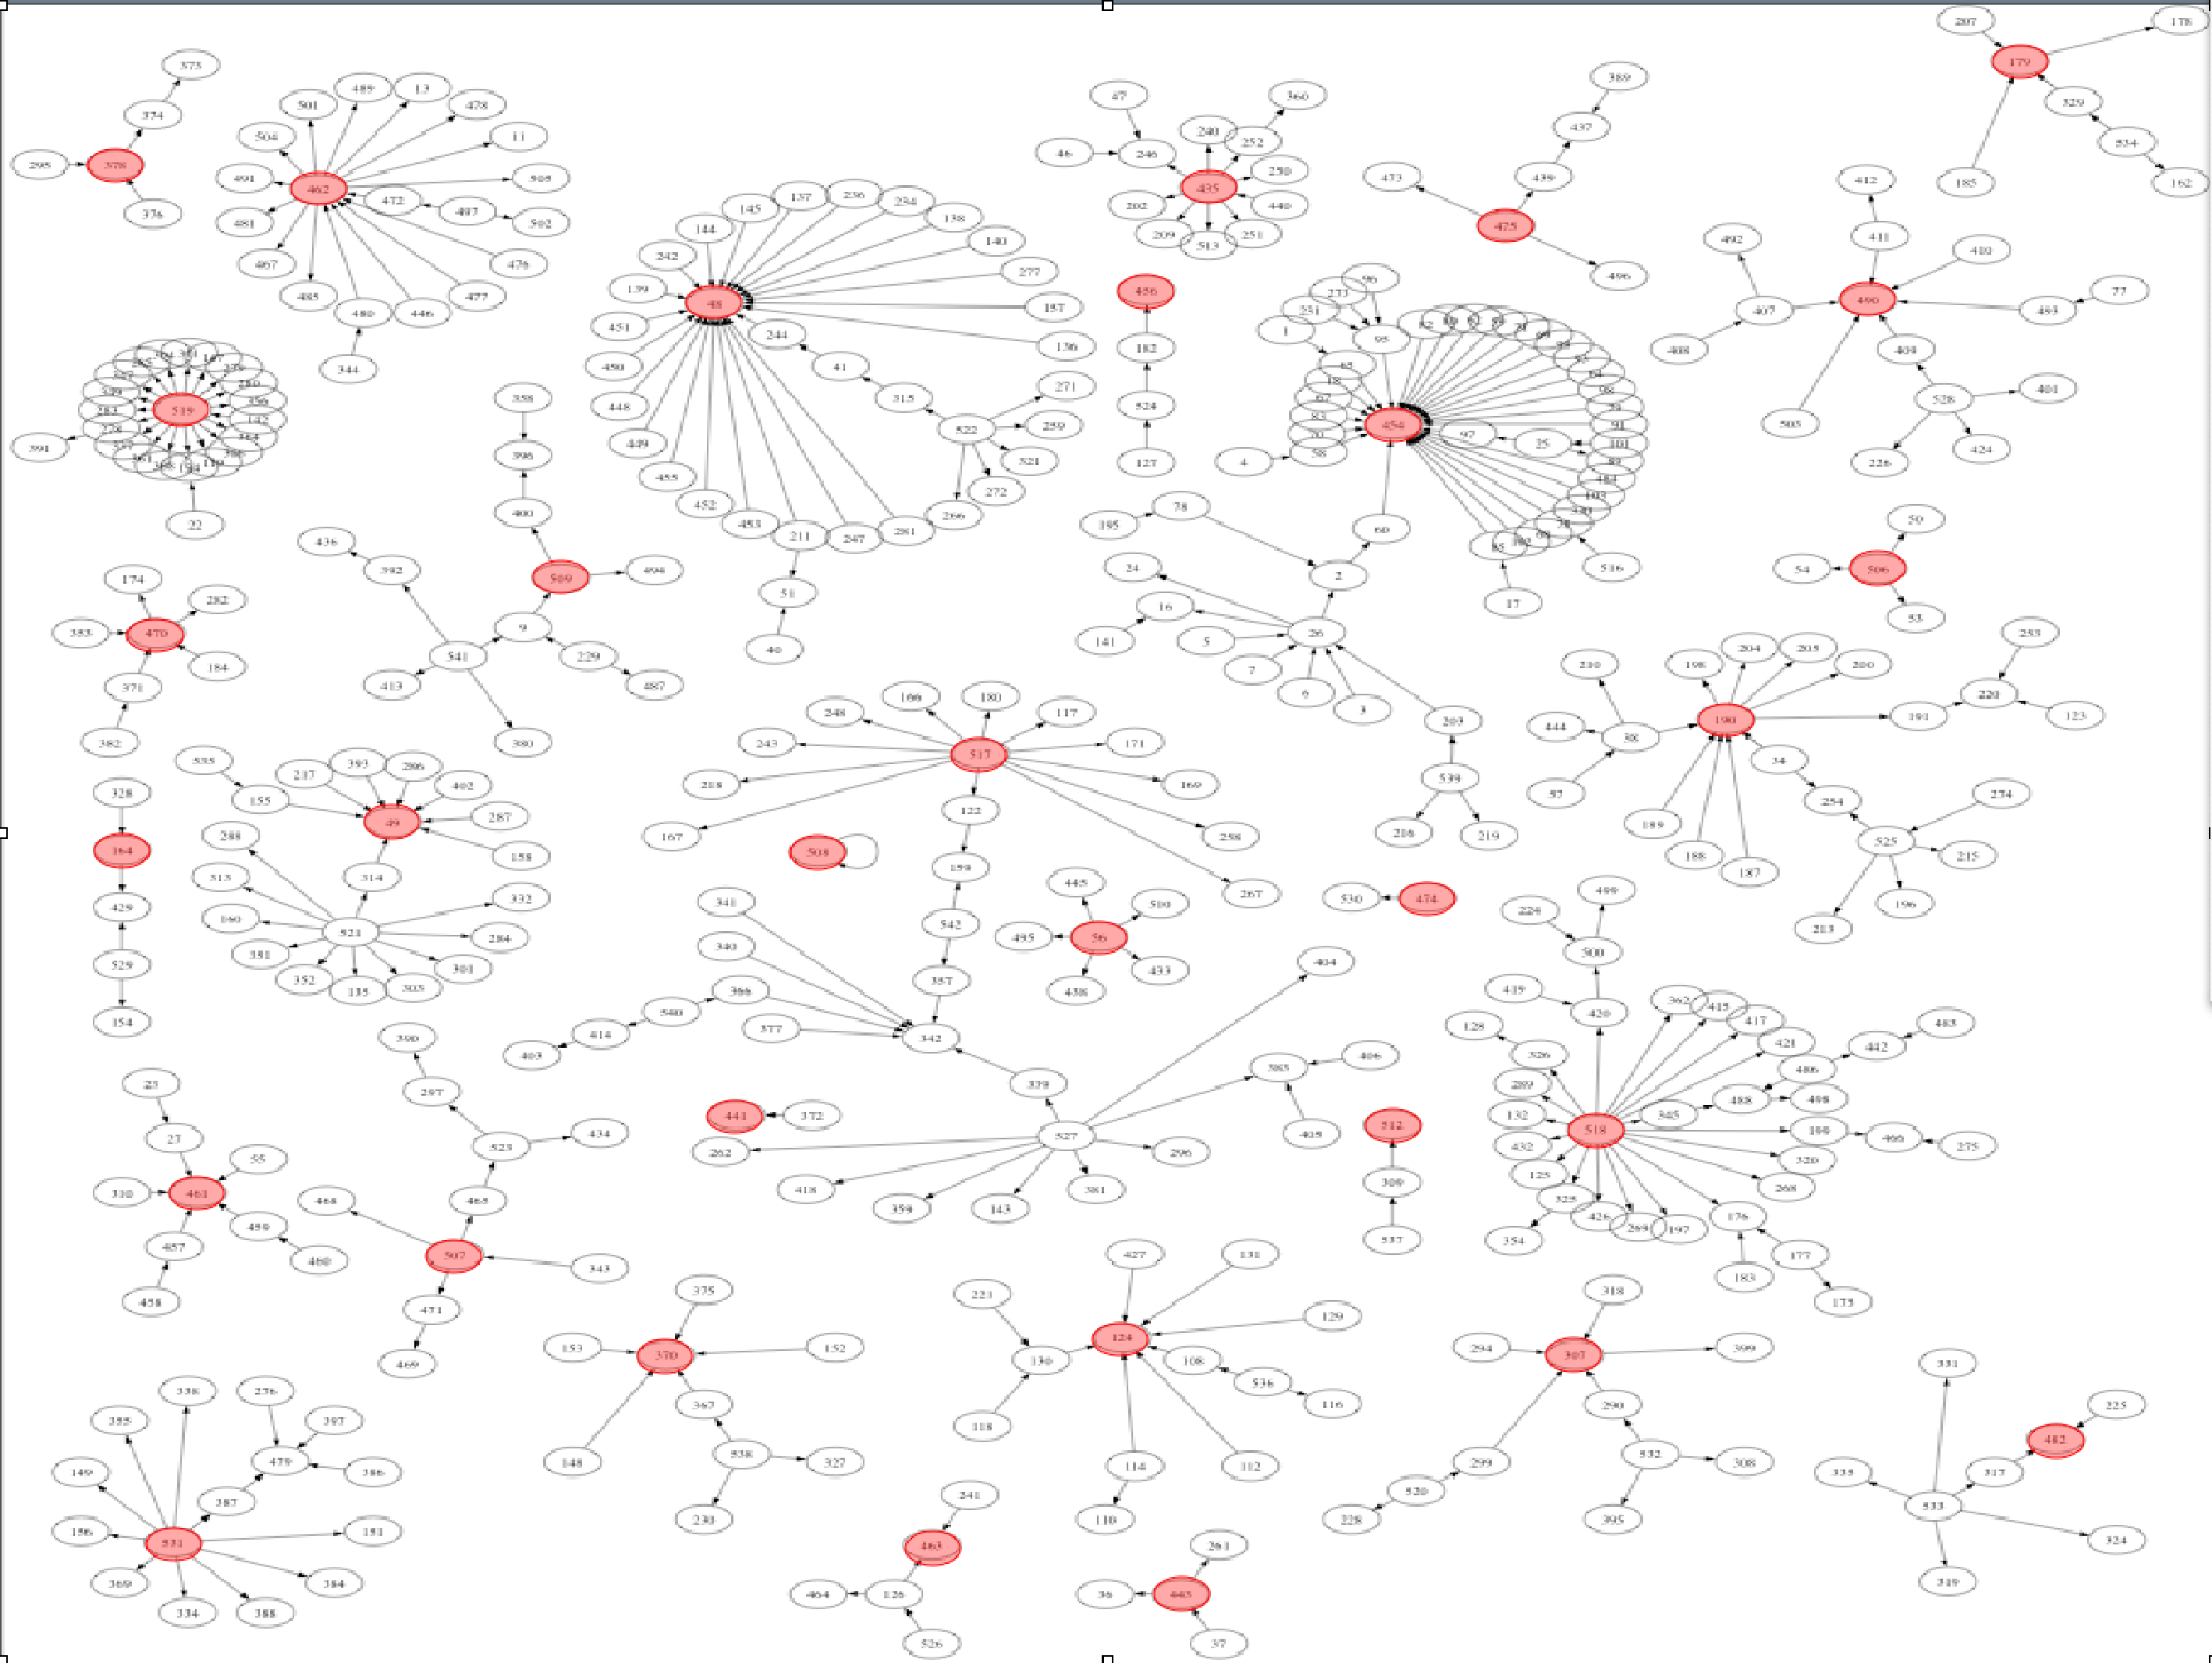
\includegraphics[width=.65\linewidth]{clusternetwork.pdf}
    \end{center}
  \end{frame}


\section{Transformations of Spatial Data}
\subsection{Area to Point}
\begin{frame}
  \frametitle{Area to Point Transformation: Centroids}
    \begin{center}
      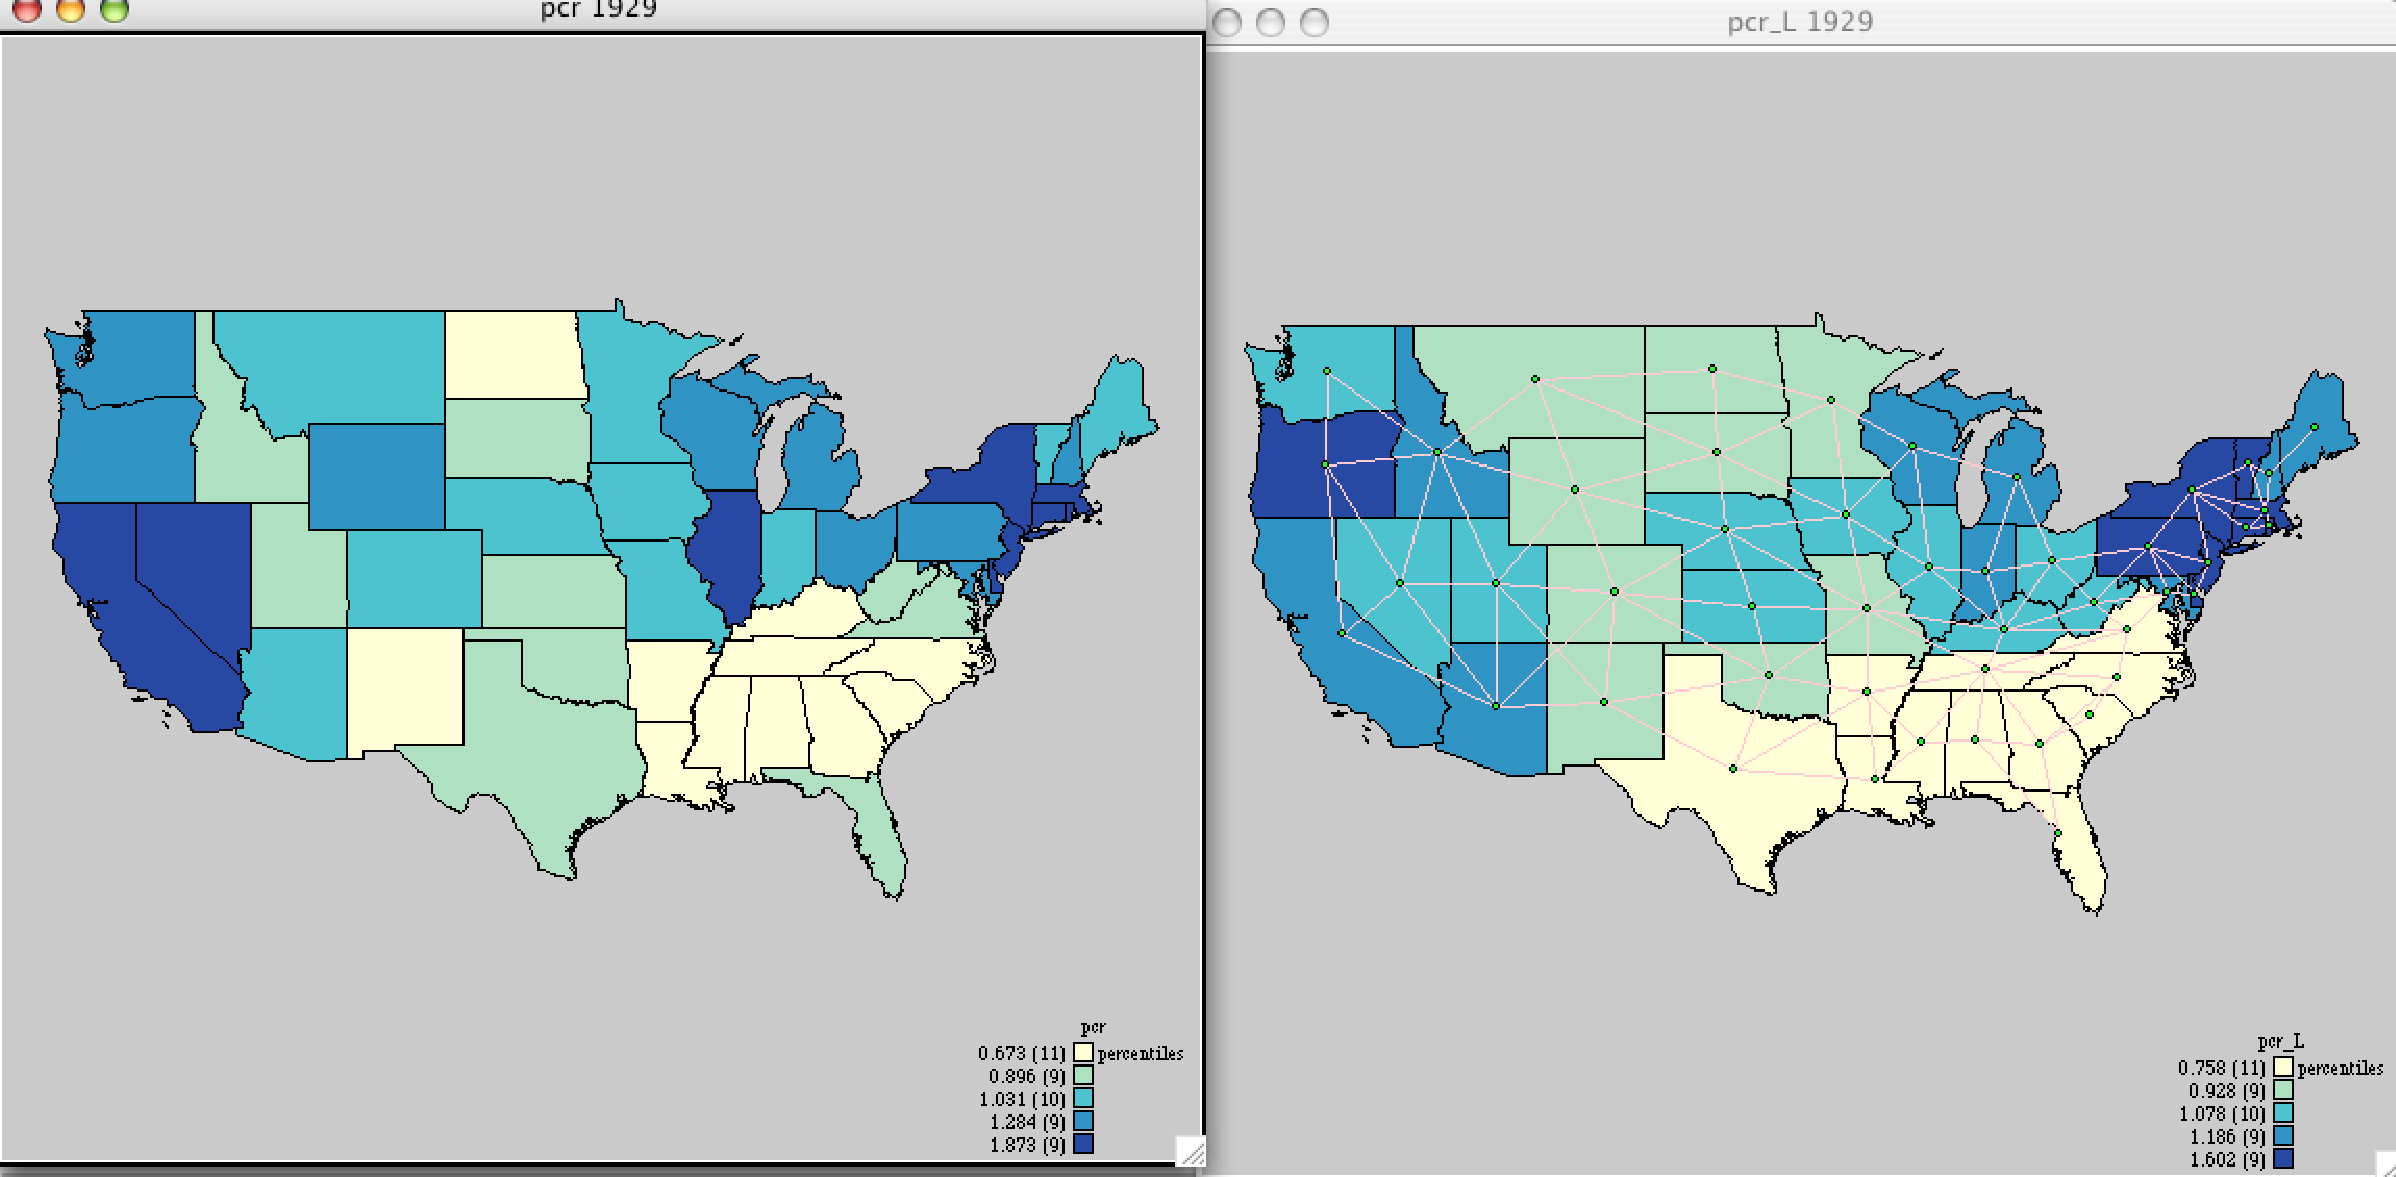
\includegraphics[width=.65\linewidth]{area2point}
    \end{center}
  \end{frame}

\subsection{Point to Area}
\begin{frame}
  \frametitle{Point to Area Transformation: Thiessen Polygons}
    \begin{center}
      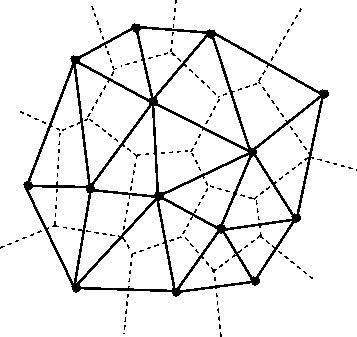
\includegraphics[width=.65\linewidth]{dt.jpg}
    \end{center}
  \end{frame}



\subsection{Change of Support Problem}
\begin{frame}[<+->]
  \frametitle{Change of Support Problem}
  \begin{block}{Transformation from one spatial framework to another}
    \begin{itemize}
      \item Point data to area data
      \item Regional data: areal interpolation
    \end{itemize}
   \end{block}
   \begin{block}{Scaling}
    \begin{itemize}
      \item Upscaling: points to areas or, areas to larger areas 
      \item Downscaling: larger areas to smaller composite areas
    \end{itemize}
   \end{block}

    \end{frame}

\begin{frame}[<+->]
  \frametitle{Change of Support Problem: Point to Area}

\begin{block}{Example}
     \begin{itemize}
       \item Estimate soil contamination for a census tract given point
	 samples in  the tract.
       \item Sample points $(s(1),\ldots,s(n))$ are the supports
       \item Prediction is for the area $(A)$, $Y(A)$
     \end{itemize}
    \end{block}

\begin{block}{Estimation}
     \begin{itemize}
       \item Assume a constant mean (contamination), then $E[Y(i)]=\mu \ \forall i$ 
       \item Simple estimator: $\hat{Y} = (1/n) \sum_{i=1}^n y(i)$
       \item Problems
	 \begin{itemize}
	   \item Ignores spatial correlation in $Y(i)$ over the sites
	   \item Ignores the difference in variances: $V(Y(A)) < V(\hat{Y})$
	   \item May significantly over or under estimate $Y(A)$
	   \item Geostatistical methods are better
	 \end{itemize}
     \end{itemize}
    \end{block}
  \end{frame}
 
 \begin{frame}[<+->]
  \frametitle{Change of Support Problem: Areal Interpolation}

\begin{block}{Example}
     \begin{itemize}
       \item Census tracts from 2000 and 1990
       \item Due to population growth, some 1990 tracts may have been split
     \end{itemize}
    \end{block}
\begin{block}{}
    \begin{center}
      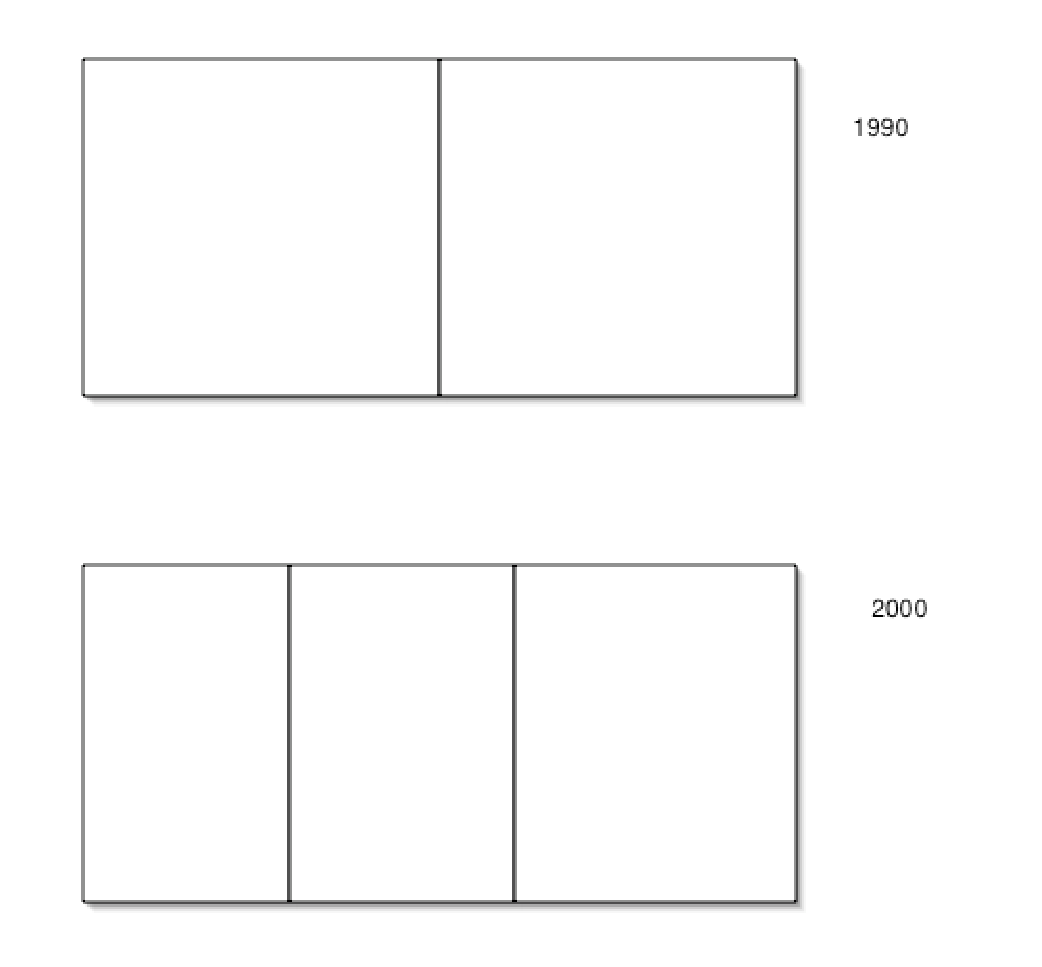
\includegraphics[width=.45\linewidth]{arealinterpolation}
    \end{center}
\end{block}
  \end{frame}

 \begin{frame}[<+->]
 \frametitle{Change of Support Problem: Areal Interpolation}
\begin{block}{Methods}
     \begin{itemize}
       \item Cartographic based
       \item Statistical based
     \end{itemize}
    \end{block}
\begin{block}{Cartographic}
  \begin{itemize}
    \item Polygon overlap
    \item Adjacency information to smooth
  \end{itemize}
\end{block}
\begin{block}{Statistical}
  \begin{itemize}
    \item Fit models to surface data on ancillary variables
    \item Use models to interpolate
  \end{itemize}
\end{block}

  \end{frame}
 
\end{document}

